\chapter{Pianificazione di traiettorie}
L'obiettivo della pianificazione di traiettorie è quello di generare ingressi di riferimento per il sistema di controllo del moto che assicuri l'esecuzione da parte del manipolatore delle traiettorie pianificate. Definiamo:
\begin{itemize}
	\item \textbf{Percorso:} è il luogo dei punti dello spazio operativo che il manipolatore deve descrivere nell'esecuzione del movimento assegnato. Pertanto la descrizione è di tipo \emph{geometrica}.
	\item \textbf{Traiettoria:} è un \emph{percorso} su cui sia specificata una \underline{legge oraria} di moto.
\end{itemize}
In linea di principio, un \emph{algoritmo} di pianificazione della traiettoria avrà il seguente schema
\begin{center}
	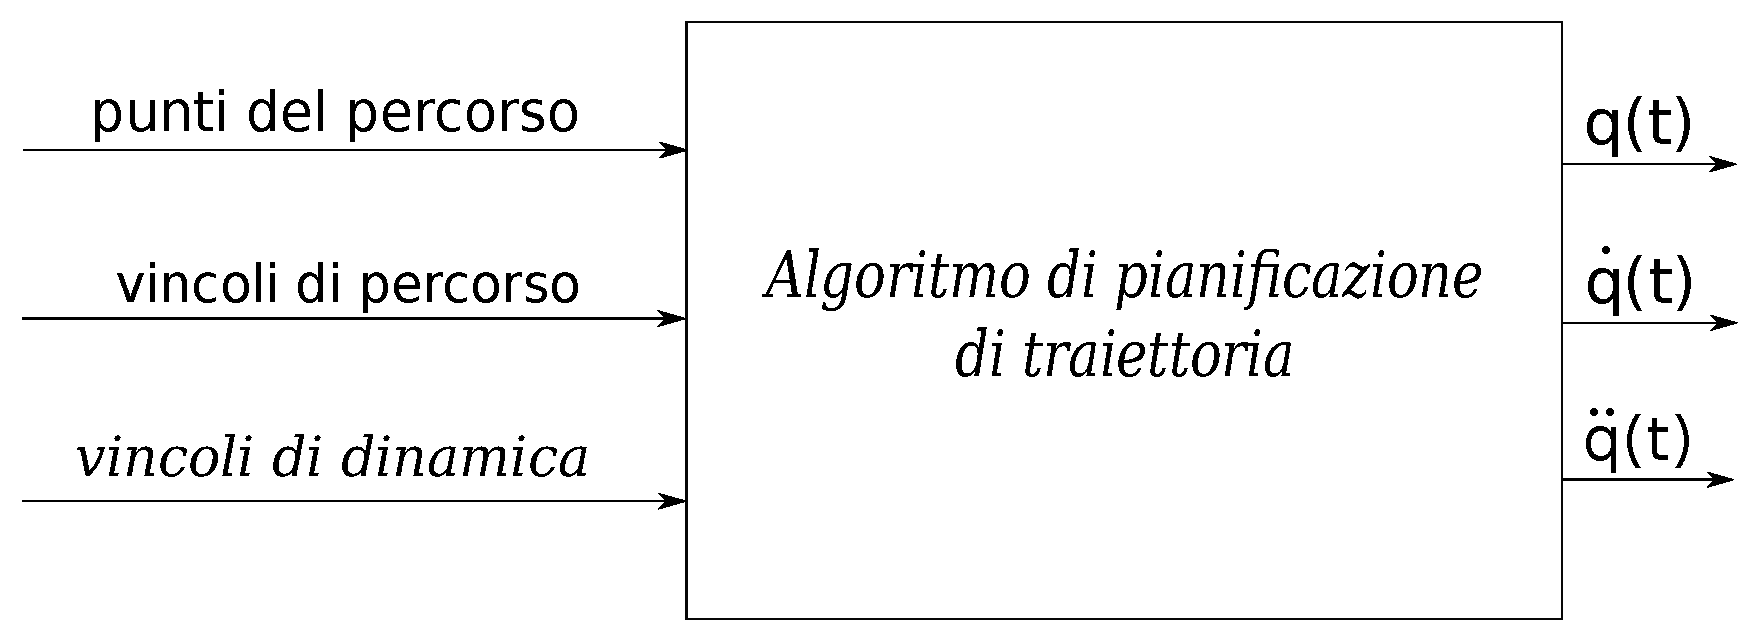
\includegraphics[scale=0.3]{algoritmoTraiettorie.pdf}
\end{center}
dove l'uscita è rappresentata dalle traiettorie dell'organo terminale espresse come sequenze di posa, velocità e accelerazione. Questo algoritmo generico, può operare nello spazio dei giunti che in quello operativo.

\section{Spazio dei giunti}
La specificazione di un particolare movimento viene usualmente effettuata assegnando, nello \emph{spazio operativo}, alcuni parametri della traiettoria, come
\begin{itemize}
	\item posa iniziale e finale dell'organo terminale,
	\item eventuali pose intermedie dell'organo terminale,
	\item tempi di percorrenza di alcuni percorsi geometrici.
\end{itemize}
Se si vuole pianificare una traiettoria nello \emph{spazio dei giunti}, a partire dalle posiziono e dagli orientamenti assegnati all'organo terminale bisogna preventivamente ricavare i valori delle variabili di giunti corrispondenti alle pose fissate dall'utente.

\paragraph{}
L'algoritmo di pianificazione genera una funzione $\underline{q}(t)$ che interpola i valori assegnati per le variabili di giunto nel rispetto dei vincoli imposti. In generale all'algoritmo si richiedono le seguenti caratteristiche:
\begin{itemize}
	\item Necessariamente:
	\begin{itemize}
		\item $q(t)$ funzione continua
		\item $\dot{q}(t)$ funzione continua
	\end{itemize}
	\item Se riusciamo, vogliamo anche:
	\begin{itemize}
		\item $\ddot{q}(t)$ funzione continua
		\item la funzione $Jerk$, definita come $j(t) = \frac{d}{dt} \ddot{q}(t)$ limitata
	\end{itemize}
\end{itemize}
ovvero, gli obiettivi della pianificazione delle traiettorie.


\subsection{Moto punto-punto}
Il manipolatore deve muoversi da una configurazione iniziale di variabili di giunto, ad una configurazione finale in un tempo fissato. Pertanto, si richiede di portare la variabile angolare $q$ da un valore iniziale $q_i$ ad un valore finale $q_f$ in un intervallo di tempo $t_f$. Chiaramente, si possono individuare infinite funzioni che compiono questo tragitto
\begin{center}
	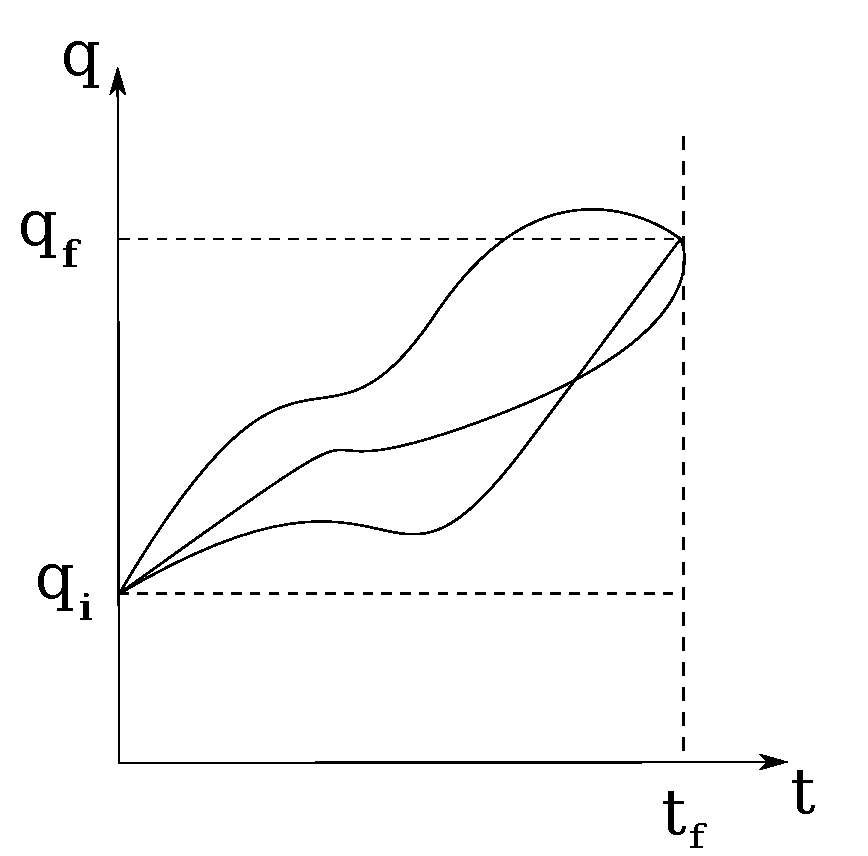
\includegraphics[scale=0.3]{infiniteConfigurazioni.pdf}
\end{center}
ma l'algoritmo dovrà generare una traiettoria che vada a ottimizzare, in relazione ad un qualche \emph{indice di qualità}, lo spostamento di $q$.

\paragraph{}
Andiamo a modellare il sistema con
\begin{equation}
	I\ddot{q} = \tau
\end{equation}
e impostiamo un problema di ottimo vincolato, ovvero cerchiamo $\dot{q}(t)$ tale che
\begin{itemize}
	\item minimizzi l'indice di qualità $\int_0^{t_f} \tau^2(\sigma) d \sigma$
	\item soddisfi il vincolo $\int_0^{t_f} \dot{q}(\sigma) d \sigma  = q_f - q_i$
\end{itemize}
il risultato è che $q(t)$ sarà un \emph{polinomio cubico}, ovvero con \emph{velocità parabolica}. 
\subsubsection{\underline{Profilo Parabolico:}}
Risulta quindi,
\begin{align}
	q(t) = a_3 t^3 + a_2 t^2 + a_1 t + a_0 \\
	\dot{q}(t) = 3 a_3 t^2 + 2 a_2 t + a_1 \\
	\ddot{q}(t) = 6 a_3 t + 2 a_2
\end{align}

\begin{center}
	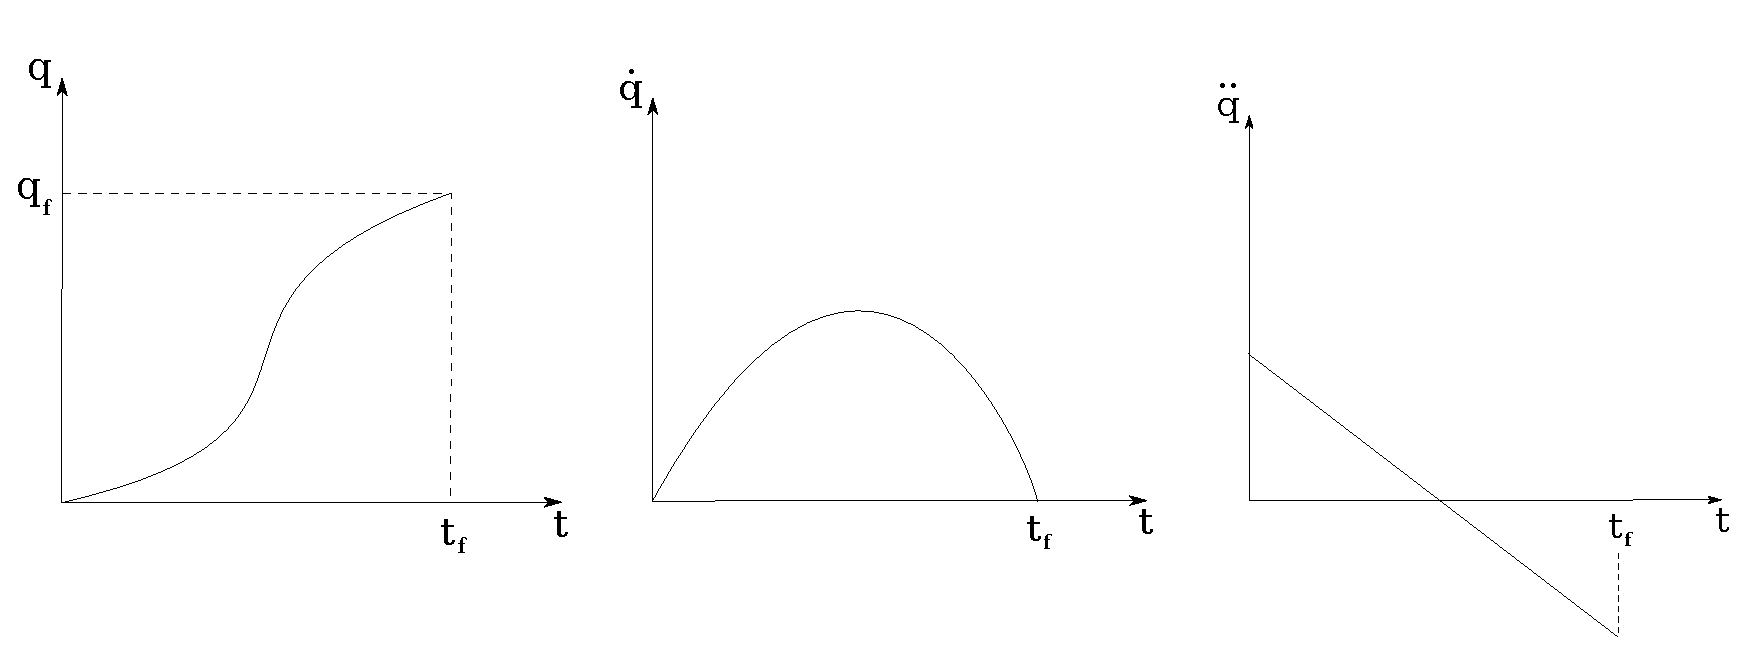
\includegraphics[scale=0.3]{velocitaParabolica.pdf}
	\caption{Andamento temporale con legge oraria della velocità parabolica.}
\end{center}
Abbiamo quindi, guardando la ($10.2$), quattro coefficienti $a_0$, $a_1$, $a_2$ e $a_3$ su cui possiamo lavorare e andare a imporre $q_i$, $q_f$, $\dot{q}_i$ e $\dot{q}_f$. Non possiamo imporre nulla sulle accelerazioni. In quel caso, dobbiamo usare un polinomio di quinto grado per $q(t)$.

\subsubsection{\underline{Profilo Trapezoidale:}}
Un approccio alternativo con leggi orarie di tipo polinomiale \emph{misto} che viene adottato spesso nella pratica industriale è quello del \emph{profilo trapezoidale di velocità}, che impone un'accelerazione costante nella fase di partenza, una velocità di crociera e una decelerazione costante nella fase di arrivo.

La traiettoria che ne risulta è costituita da un tratto lineare \emph{raccordato} con due tratti parabolici nell'intorno della posizione finale e iniziale.

\begin{center}
	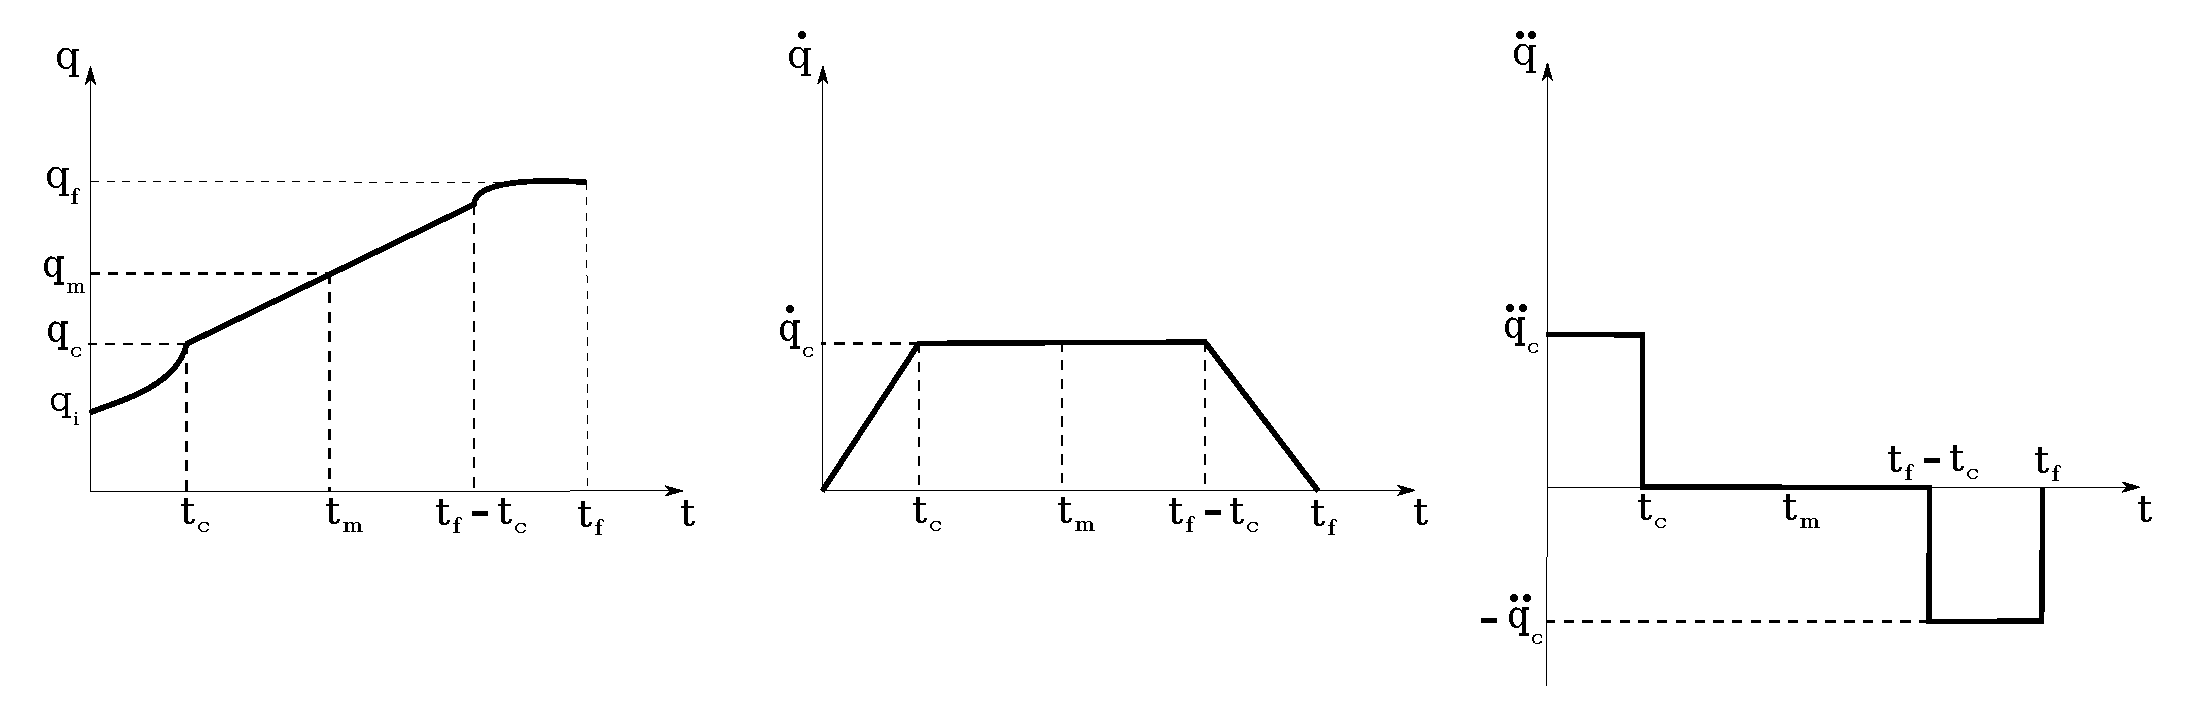
\includegraphics[scale=0.3]{velocitaTrapezoidale.pdf}
	\caption{Andamento temporale con legge oraria trapezoidale della velocità.}
\end{center}
nei grafici abbiamo supposto che la velocità iniziale e finale siano nulle. Vediamo adesso i \emph{metodi di pianificazione} del profilo di velocità trapezoidale,
\begin{itemize}
	\item \textbf{Assegnati $q_i$, $q_f$, $t_f$, $\ddot{q}_c$ :} vogliamo rispettare il vincolo sull'area del trapezio, otteniamo pertanto
		\begin{equation*}
			\int_0^{t_f} \dot{q}(\sigma) d\sigma = q_f - q_i \quad \Rightarrow \quad 
			\begin{cases}
				q_f - q_i = (t_f - t_c) \dot{q}_c \\
				\dot{q}_c = \ddot{q}_c t_c 
			\end{cases}
			\quad \Rightarrow \quad q_f - q_i = \ddot{q}_c t_f t_c - \ddot{q}_c t_c^2
		\end{equation*}
		e quindi 
		\begin{equation*}
			t_c^2 - t_f t_c +  \frac{q_f - q_i}{\ddot{q}_c} = 0 \quad \Rightarrow \quad t_c = \frac{t_f}{2} \pm \frac{\sqrt{t_f^2 - 4 \frac{q_f - q_i}{\ddot{q}_c}}}{2}
		\end{equation*}
		guardando il dominio naturale della radice,
		\begin{equation*}
			t_f^2 \geqslant 4 \frac{q_f - q_i}{\ddot{q}_c} \quad \Rightarrow \quad \vert \ddot{q}_c \vert \geqslant 4 \frac{\vert q_f - q_i \vert}{t_f^2}
		\end{equation*}
		e notiamo che se scegliamo l'accelerazione con l'uguaglianza
		\begin{equation}
			\vert \ddot{q}_c \vert = 4 \frac{\vert q_f - q_i \vert}{t_f^2}
		\end{equation}
		otteniamo un \emph{profilo triangolare di velocità}, perchè la traiettoria \underline{non} presenta il tratto a velocità costante, ma solo i tratti di accelerazione e decelerazione. Pertanto, avendo $q_i$, $q_f$, $t_f$, calcolando $\ddot{q}_c$ e $t_c$ si generano le funzioni polinomiali seguenti
		\begin{equation}
			q(t) = 
			\begin{cases}
				q_i + \frac{1}{2} \ddot{q}_c t^2 \qquad \qquad \;\;\; 0 \leqslant t \leqslant t_c \\
				q_i + \ddot{q}_c t_c (t- \frac{t_c}{2}) \qquad t_c < t \leqslant t_f - t_c \\
				q_i - \frac{1}{2} \ddot{q}_c (t_f - t)^2 \qquad t_f - t_c < t \leqslant t_f
			\end{cases}
		\end{equation}			
	
	\item \textbf{Assegnati $q_i$, $q_f$, $t_f$, $\dot{q}_c$ :} Anche in questo caso partiamo dal vincolo, ma stavolta non esplicitiamo $\dot{q}_c$ perchè non abbiamo l'accelerazione,
		\begin{equation*}
			(t_f - t_c) \dot{q}_c = q_f - q_i \quad \Rightarrow \quad t_f - t_c = \frac{q_f - q_i}{\dot{q}_c} \quad \Rightarrow \quad t_c = t_f - \frac{q_f - q_i}{\dot{q}_c}
		\end{equation*}
		a questo punto guardando la Figura 10.2 notiamo due cose:
		\begin{enumerate}
			\item $t_c > 0$, ovvero
				\begin{equation*}
					t_f > \frac{q_f - q_i}{\dot{q}_c} \quad \Rightarrow \quad \vert \dot{q}_c \vert > \frac{\vert q_f - q_i \vert}{t_f}
				\end{equation*}
			\item $t_c \leqslant \frac{t_f}{2}$, ovvero
				\begin{equation*}
					t_f - \frac{q_f - q_i}{\dot{q}_c} \leqslant \frac{t_f}{2} \quad \Rightarrow \quad \vert \dot{q}_c \vert \leqslant 2 \frac{\vert q_f - q_i \vert}{t_f}
				\end{equation*}
		\end{enumerate}
		quindi otteniamo,
		\begin{equation}
			\frac{\vert q_f - q_i \vert}{t_f} < \vert \dot{q}_c \vert \leqslant 2 \frac{\vert q_f - q_i \vert}{t_f}
		\end{equation}
		e quindi possiamo ricavare $t_c$ e $\ddot{q}_c$ riconducendoci alle equazioni ($10.6$).
	\item \textbf{Assegnati $q_i$, $q_f$, $\dot{q}_c$, $\ddot{q}_c$ :} In questo caso, abbiamo
		\begin{equation}
			\dot{q}_c = \ddot{q}_c t_c \quad \Rightarrow \quad t_c = \frac{\dot{q}_c}{\ddot{q}_c} 
		\end{equation}
		ma l'accelerazione è discontinua e pertanto il Jerk è infinito. Spesso è preferibile ammorbidire la fase di accelerazione utilizzando, ad esempio le \emph{S-curve}. Il grafico del trapezio risulta più morbido nei punti di raccordo.
\end{itemize}

\subsection{Sequenza di punti}
Affrontiamo adesso, il problema di generazione della traiettoria quando siano specificati $N$ punti di cammino (\emph{waypoint}), che devono essere raggiunti dal manipolatore in determinati istanti. In linea di principio si può pensare di usare un solo polinomio di grado $N-1$ che passi per tutti i punti. Ma abbiamo svariati problemi,
\begin{itemize}
	\item Non possiamo assegnare velocità iniziale e finale.
	\item Più il grado aumenta e più aumenta il suo carattere oscillatorio.
	\item Sistema di calcolo oneroso, ecc...
\end{itemize}
pertanto, invece di considerare un singolo polinomio di grado elevato, andiamo a considerare un \emph{insieme di polinomi interpolatori} di grado più basso uniti tra di loro nei punti di cammino. Abbiamo visto precedentemente che il grado più basso è il terzo perchè ci garantisce la continuità della velocità nei punti di cammino.

\paragraph{} 
Facendo riferimento ad una singola variabile di giunto, si deve individuare una funzione $q(t)$, costituita da una sequenza di polinomi cubici
\begin{equation}
	\Pi_k(t) \quad \dot{\Pi}_k(t) \quad \ddot{\Pi}_k(t) \qquad  k = 1, \cdots, N-1
\end{equation}
che assuma valori $q_k$ per $t = t_k$ ($k = 1, \cdots, N$) con $q_1 = q_i$, $t_1 = 0$, $q_N = q_f$, $t_N = t_f$. 
\begin{center}
	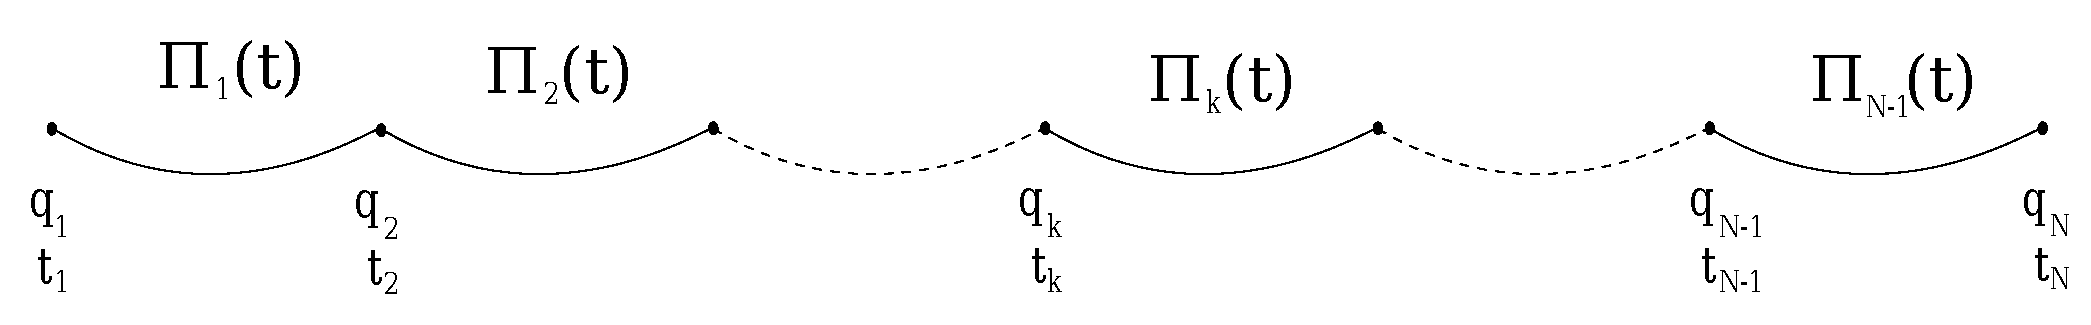
\includegraphics[scale=0.3]{traiettoria.pdf}
	\caption{Waypoint}
\end{center}
con il generico polinomio $\Pi_k(t)$ che raccorda $q_k$ con $q_{k+1}$. I valori di $\dot{q}(t)$ in corrispondenza dei punti di cammino possono essere scelti arbitrariamente. Ma possiamo effettuare una scelta più saggia, indicando con $v_k$ la pendenza della spezzata nell'intervallo di tempo $[t_{k-1}, t_k]$
\begin{equation}
	v_k = \frac{(q_k - q_{k-1})}{(t_k - t_{k-1})}
\end{equation}
utilizziamo le seguenti regole:
\begin{equation}
	\begin{cases}
		\dot{q}_1 = 0 \\
		\dot{q}_N = 0 \\
		\dot{q}_k = 
		\begin{cases}
			0 \qquad \qquad \qquad \quad \text{con $v_k$, $v_{k+1}$ discordi} \\
			\frac{1}{2} (v_k + v_{k+1}) \qquad \text{con $v_k$, $v_{k+1}$ concordi}
		\end{cases}
	\end{cases}
\end{equation}

\paragraph{}
Adesso andiamo a porre le condizioni iniziali,
\begin{equation}
	\begin{cases}
		\Pi_1(t_1) = q_1 \\
		\dot{\Pi}_1(t_1) = 0 \\
		\ddot{\Pi}_1(t_1) = 0 
	\end{cases}
	\qquad
	\begin{cases}
		\Pi_{N-1}(t_N) = q_N \\
		\dot{\Pi}_{N-1}(t_N) = 0 \\
		\ddot{\Pi}_{N-1}(t_N) = 0 
	\end{cases}
\end{equation}
e per ogni $k \in (1,N)$ \emph{punti intermedi} scriviamo quattro equazioni:
\begin{itemize}
	\item Una equazione di passaggio per $q_k$.
	\item Tre equazioni che pongono le \emph{condizioni di continuità} della posizione, velocità e accelerazione.
\end{itemize}
e risulta
\begin{equation}
	\begin{cases}
		\Pi_{k-1}(t_k) = q_k \\
		\Pi_{k-1}(t_k) = \Pi_{k}(t_k) \\
		\dot{\Pi}_{k-1}(t_k) = \dot{\Pi}_{k}(t_k) \\
		\ddot{\Pi}_{k-1}(t_k) = \ddot{\Pi}_{k}(t_k)
	\end{cases}
\end{equation}
e si ottengono pertanto $4N-2$ equazioni nei $4(N-1)$ coefficienti incogniti. Per rendere il sistema \emph{quadrato} perchè vogliamo usare solo polinomi di terzo grado, andiamo ad aggiungere due \emph{punti virtuali} su cui è possibile imporre vincoli di continuità su posizione, velocità e accelerazione. Notiamo come \emph{non} importa la collocazione di questi due punti virtuali in quanto andiamo a imporre vincoli solo sulla continuità. 

Consideriamo quindi $N+2$ istanti di tempo $t_k$, dove $t_2$ e $t_{N+1}$ individuano convenzionalmente i punti virtuali introdotti. Otteniamo,

\begin{equation}
t_2: 
\begin{cases}
	\Pi_1(t_2) = \Pi_2(t_2) \\
	\dot{\Pi}_1(t_2) = \dot{\Pi}_2(t_2) \\
	\ddot{\Pi}_1(t_2) = \ddot{\Pi}_2(t_2) 
\end{cases}
\;
t_{N+1}:
\begin{cases}
	\Pi_N(t_{N+1}) = \Pi_{N+1}(t_{N+1}) \\
	\dot{\Pi}_N(t_{N+1}) = \dot{\Pi}_{N+1}(t_{N+1}) \\
	\ddot{\Pi}_N(t_{N+1}) = \ddot{\Pi}_{N+1}(t_{N+1})
\end{cases}
\end{equation}
ne risulta un sistema di $4(N+1)$ equazioni per la determinazione dei $4(N+1)$ coefficienti degli $N+1$ polinomi cubici.

\section{Spazio operativo}
Con la pianificazione di traiettorie nello spazio dei giunti si genera, sulla base di primitive di movimento, una sequenza temporale dei valori che le variabili giunto $q(t)$ devono assumere in modo che il manipolatore si porti dalla configurazione iniziale a quella finale, passando eventualmente attraverso una serie di configurazioni intermedie.

Quando si desidera che il moto si sviluppi su un percorso di caratteristiche geometriche definite nello \emph{spazio operativo}, è necessario pianificare le traiettorie direttamente nello stesso spazio. 

\subsection{Posizione}
La pianificazione desiderata viene descritta attraverso una curva parametrica definita dall'ascissa curvilinea $s$. Pertanto, la posizione viene descritta come $\underline{p}=\underline{p}(s)$, ovvero una curva generica nello spazio con
\begin{itemize}
	\item \emph{Vettore tangenziale}: $\underline{t} = \frac{d \underline{p}}{ds}$
	\item \emph{Versore normale}: $\underline{n} = \frac{1}{\Vert \frac{d^2 \underline{p}}{d s^2} \Vert } \frac{d^2 \underline{p}}{ds^2}$
	\item \emph{Versore binormale}: $\underline{b} = \underline{t} \times \underline{n}$
\end{itemize}

\begin{center}
	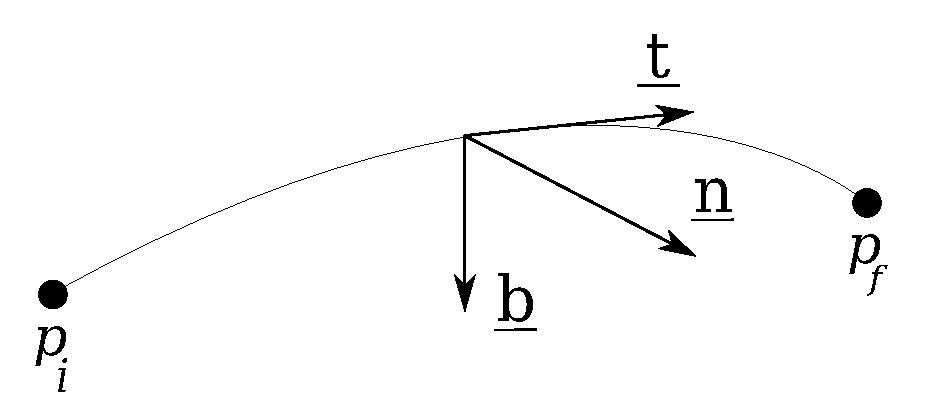
\includegraphics[scale=0.3]{rappresentazionePrametrica.pdf}
	\caption{Rappresentazione parametrica di una curva nello spazio.}
\end{center}

\subsubsection{\underline{Segmento nello spazio}}
Supponiamo un percorso rettilineo da $\underline{p}_i$ a $\underline{p}_f$. Sia $L$ la lunghezza della traiettoria, $L = \Vert \underline{p}_f - \underline{p}_i$, chiaramente, vale $0 \leqslant s \leqslant L$. Pertanto,
\begin{equation}
	\underline{p}(s) = \underline{p}_i + \frac{\underline{p}_f - \underline{p}_i}{\Vert \underline{p}_f - \underline{p}_i \Vert} s = \underline{p}_i + \underline{t}s
\end{equation} 
con $\underline{t} = \frac{\underline{p}_f - \underline{p}_i}{\Vert \underline{p}_f - \underline{p}_i \Vert}$, inoltre,
\begin{align}
	\dot{\underline{p}}(s) = \frac{d p}{ds} \cdot \frac{ds}{dt} = \underline{t} \dot{s} \\
	\ddot{\underline{p}}(s) = \frac{d p}{ds} \cdot \frac{d^2s}{dt^2} = \underline{t} \ddot{s}
\end{align}

\subsubsection{\underline{Circonferenza nello spazio}}
Supponendo che la traiettoria sia un arco di circonferenza, per la rappresentazione parametrica dobbiamo definire i parametri significativi,
\begin{itemize}
	\item Il vettore posizione $\underline{p}_i$ che indica in punto iniziale dell'arco, nonché un punto appartenente alla circonferenza.
	\item Il vettore posizione di un punto dell'asse della circonferenza e il versore di tale asse $(\underline{d}, \underline{r})$.
	\item Lunghezza dell'arco $S$, chiaramente si ha $0 \leqslant s < S$.
	\item Sia $\underline{\delta} = \underline{p}_i - \underline{d}$, definiamo il vettore che indica il centro della circonferenza come $\underline{c} = \underline{d} + (\underline{\delta}^T \underline{r})\underline{r}$.
\end{itemize}
definiamo una \emph{terna} $\langle c \rangle$ con origine nel centro della circonferenza, con $z' \parallel \underline{r}$, asse $x'$ passante per $\underline{p}_i$ e con $\rho = \Vert \underline{p}_i - \underline{c} \Vert$ 
\begin{center}
	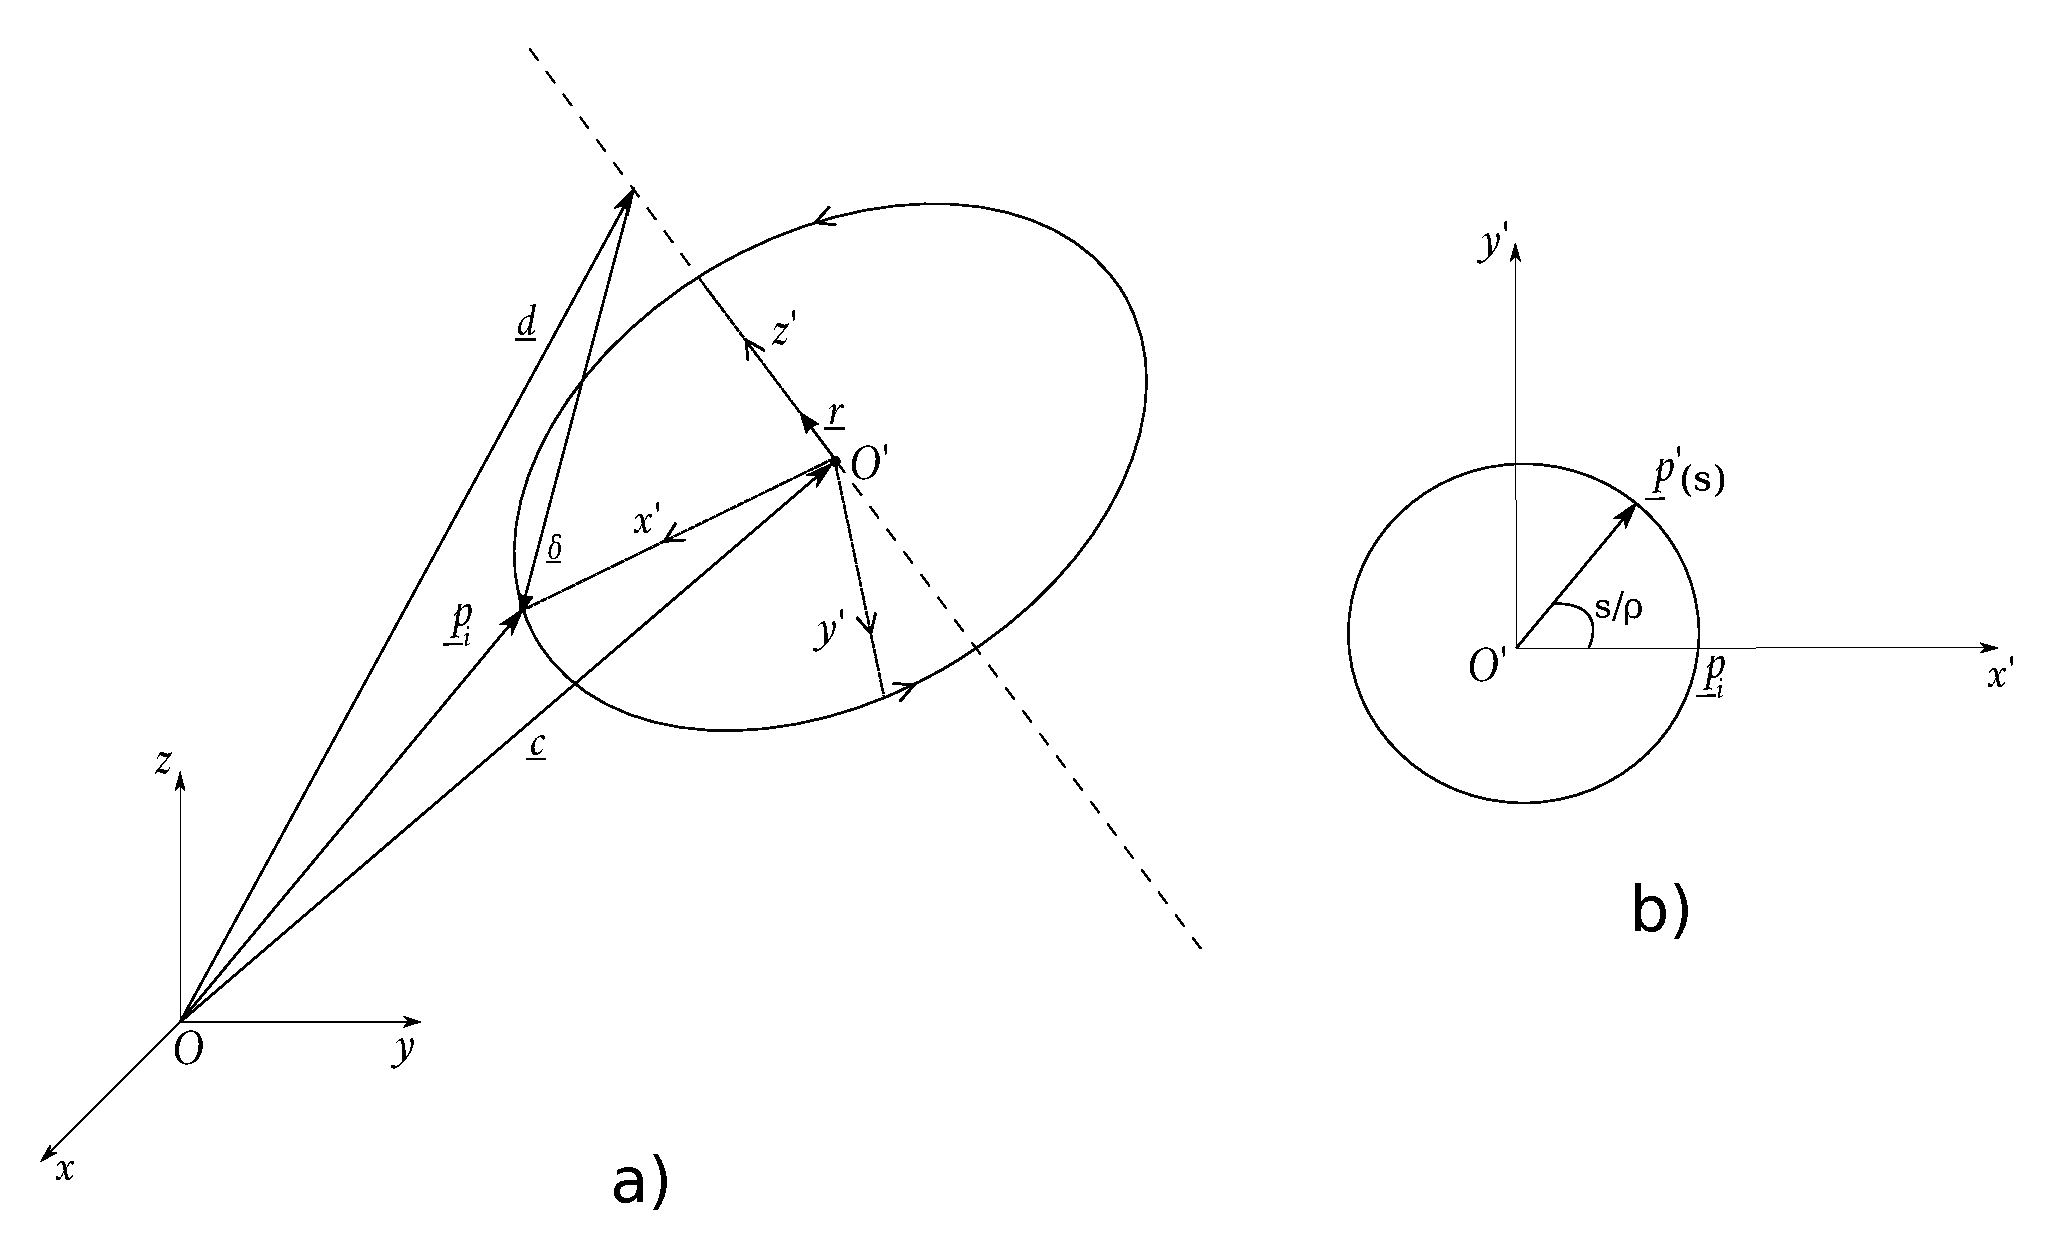
\includegraphics[scale=0.3]{traiettoriaCirconferenza.pdf}
	\caption{a) Rappresentazione parametrica b) Vista del piano $x'y'$}
\end{center}
quindi definiamo i versori,
\begin{equation}
	i' = \frac{\underline{p}_i - \underline{c}}{\Vert \underline{p}_i - \underline{c}\Vert} \qquad k' = \underline{r} \qquad j' = k' \times i'
\end{equation} 
e guardando sul piano $x'y'$ in Figura b), definiamo per la nuova terna
\begin{equation}
	\rho '(s) = \rho 
	\begin{bmatrix}
		\cos (\frac{s}{\rho}) \\
		\sin (\frac{s}{\rho}) \\
		0
	\end{bmatrix}
\end{equation}
e definendo la matrice di rotazione $R = 
\begin{bmatrix}
	i' & j' & k'
\end{bmatrix} $, in terna base otteniamo,
\begin{equation}
	\underline{p}(s) = \underline{c} + R \underline{p}'(s)
\end{equation}

Scriviamo adesso $\underline{t}$ e $\underline{n}$ che mi servono per scrivere la velocità e l'accelerazione,
\begin{equation}
	\underline{t} = R \underline{t}' = R
	\begin{bmatrix}
		- \sin(\frac{s}{\rho}) \\
		\cos(\frac{s}{\rho}) \\
		0
	\end{bmatrix},
	\qquad
	\underline{n} = R \underline{n}' = R
	\begin{bmatrix}
		- \cos(\frac{s}{\rho}) \\
		- \sin(\frac{s}{\rho}) \\
		0
	\end{bmatrix}
\end{equation}
e otteniamo,
\begin{align*}
	\dot{\underline{p}}(s) = \dot{s} \underline{t} = R 
	\begin{bmatrix}
		- \dot{s} \sin(\frac{s}{\rho}) \\
		\dot{s} \cos(\frac{s}{\rho}) \\
		0
	\end{bmatrix}
	\\
	\ddot{\underline{p}}(s) = \ddot{s} \underline{t} = R
	\begin{bmatrix}
		- \frac{1}{\rho} \dot{s}^2 \cos(\frac{s}{\rho}) - \ddot{s} \sin(\frac{s}{\rho}) \\
		- \frac{1}{\rho} \dot{s}^2 \sin(\frac{s}{\rho}) + \ddot{s} \cos(\frac{s}{\rho}) \\
		0
	\end{bmatrix}
\end{align*}
\newpage
\subsection{Orientamento}
Consideriamo adesso l'orientamento della \emph{terna utensile}, di solito è specificato tramite la matrice di orientazione. Ma nella fase di generazione della traiettoria, non è conveniente utilizzare tale matrice perchè non si può garantire la condizione di ortonormalità dei versori $\underline{n}$, $\underline{s}$, $\underline{a}$. 

Per risolvere questo problema, possiamo descrivere l'orientamento tramite una terna di Eulero o la descrizione Asse-angolo.

\subsubsection{\underline{Angoli di Eulero:}}
Sia $\phi_i$ l'orientazione iniziale e $\phi_f$ quella finale, possiamo descrivere un segmento in $\mathbb{R}^3$ con
\begin{equation*}
	\phi(s) = \phi_i + \frac{(\phi_f - \phi_i)}{\Vert \phi_f - \phi_i \Vert}s\, ; \quad
	\dot{\phi}(s) = \frac{(\phi_f - \phi_i)}{\Vert \phi_f - \phi_i \Vert} \dot{s} \, ; \quad
	\ddot{\phi}(s) = \frac{(\phi_f - \phi_i)}{\Vert \phi_f - \phi_i \Vert} \ddot{s}
\end{equation*}
con $s \in [0, \Vert \phi_f - \phi_i \Vert]$.

\subsubsection{\underline{Asse e Angolo:}}
Un metodo alternativo e di più chiara interpretazione nello spazio cartesiano è la rappresentazione Asse-Angolo. Assegnate due terne di coordinate nello spazio cartesiano con origini coincidenti e orientamenti diversi, è sempre possibile determinare un versore $\underline{r}$ tale che la seconda terna è ottenibile dalla prima con una rotazione di ampiezza $\vartheta_f$ intorno all'asse di tale versore.

Supponiamo di avere una terna iniziale $\langle O_i \rangle$ e una finale $\langle O_f \rangle$, caratterizzate rispettivamente dalle matrici di rotazione $R_i$ e $R_f$ rispetto alla terna base. La matrice di rotazione tra le due terne può essere calcolata, come sappiamo con
\begin{equation}
	R_f = R_i R_f^i \quad \Rightarrow \quad R_f^i = R_i^T R_f = 
	\begin{bmatrix}
		r_{11} & r_{12} & r_{13} \\
		r_{21} & r_{22} & r_{23} \\
		r_{31} & r_{32} & r_{33} 
	\end{bmatrix}
\end{equation}
Se si definisce la matrice $R^i(t)$ per descrivere la transizione tra $R_i$ e $R_f$, $R^i(t)$ deve essere tale che $R^i(0) = I$ e $R^i(t_f)= R_f^i$. Pertanto la matrice $R_f^i$ può essere espressa come matrice di rotazione intorno a un asse fisso nello spazio. Il versore $\underline{r}$ dell'asse e l'angolo $\vartheta_f$ di rotazione, possono essere calcolati per $\sin(\vartheta_f) \neq 0$ con
\begin{equation*}
	\vartheta_f = \cos^{-1} \Bigl( \frac{r_{11} + r_{22} + r_{33} - 1}{2}  \Bigr)\,; \quad
	\underline{r} = \frac{1}{2 \sin(\vartheta_f)}
	\begin{bmatrix}
		r_{32} - r_{23} \\
		r_{13} - r_{31} \\
		r_{21} - r_{12} 
	\end{bmatrix}
\end{equation*}

\paragraph{}
La matrice $R^i(t)$ può essere interpretata come una matrice $R^i(\vartheta(t), \underline{r}^i)$. Poichè $\underline{r}^i$ è costante, la velocità e l'accelerazione risultano rispettivamente
\begin{equation}
	\begin{cases}
		\underline{\omega}^i = \dot{\vartheta} \underline{r}^i \\
		\underline{\dot{\omega}}^i = \ddot{\vartheta} \underline{r}^i
	\end{cases}
\end{equation}
pertanto, per caratterizzare la traiettoria in orientamento all'organo terminale rispetto alla terna base, basta utilizzare le seguenti trasformazioni
\begin{equation}
	\begin{cases}
		R(t) = R_iR^i(t) \\
		\underline{\omega}(t) = R_i \underline{\omega}^i(t) \\
		\dot{\underline{\omega}}(t) = R_i \dot{\underline{\omega}}^i(t)
	\end{cases}
\end{equation}

Una volta specificati $\underline{p}(t)$ e $\underline{\phi}(t)$ o $R(t)$ un percorso e una traiettoria nello spazio operativo, l'applicazione di tecniche di inversione cinematica consente di ricavare le traiettorie corrispondenti $\underline{q}(t)$ nello spazio dei giunti.

 